% Options for packages loaded elsewhere
\PassOptionsToPackage{unicode}{hyperref}
\PassOptionsToPackage{hyphens}{url}
%
\documentclass[
]{article}
\usepackage{lmodern}
\usepackage{amssymb,amsmath}
\usepackage{ifxetex,ifluatex}
\ifnum 0\ifxetex 1\fi\ifluatex 1\fi=0 % if pdftex
  \usepackage[T1]{fontenc}
  \usepackage[utf8]{inputenc}
  \usepackage{textcomp} % provide euro and other symbols
\else % if luatex or xetex
  \usepackage{unicode-math}
  \defaultfontfeatures{Scale=MatchLowercase}
  \defaultfontfeatures[\rmfamily]{Ligatures=TeX,Scale=1}
\fi
% Use upquote if available, for straight quotes in verbatim environments
\IfFileExists{upquote.sty}{\usepackage{upquote}}{}
\IfFileExists{microtype.sty}{% use microtype if available
  \usepackage[]{microtype}
  \UseMicrotypeSet[protrusion]{basicmath} % disable protrusion for tt fonts
}{}
\makeatletter
\@ifundefined{KOMAClassName}{% if non-KOMA class
  \IfFileExists{parskip.sty}{%
    \usepackage{parskip}
  }{% else
    \setlength{\parindent}{0pt}
    \setlength{\parskip}{6pt plus 2pt minus 1pt}}
}{% if KOMA class
  \KOMAoptions{parskip=half}}
\makeatother
\usepackage{xcolor}
\IfFileExists{xurl.sty}{\usepackage{xurl}}{} % add URL line breaks if available
\IfFileExists{bookmark.sty}{\usepackage{bookmark}}{\usepackage{hyperref}}
\hypersetup{
  pdftitle={HW 01 - Data Visualization with ggpplot2},
  hidelinks,
  pdfcreator={LaTeX via pandoc}}
\urlstyle{same} % disable monospaced font for URLs
\usepackage[margin=1in]{geometry}
\usepackage{color}
\usepackage{fancyvrb}
\newcommand{\VerbBar}{|}
\newcommand{\VERB}{\Verb[commandchars=\\\{\}]}
\DefineVerbatimEnvironment{Highlighting}{Verbatim}{commandchars=\\\{\}}
% Add ',fontsize=\small' for more characters per line
\usepackage{framed}
\definecolor{shadecolor}{RGB}{248,248,248}
\newenvironment{Shaded}{\begin{snugshade}}{\end{snugshade}}
\newcommand{\AlertTok}[1]{\textcolor[rgb]{0.94,0.16,0.16}{#1}}
\newcommand{\AnnotationTok}[1]{\textcolor[rgb]{0.56,0.35,0.01}{\textbf{\textit{#1}}}}
\newcommand{\AttributeTok}[1]{\textcolor[rgb]{0.77,0.63,0.00}{#1}}
\newcommand{\BaseNTok}[1]{\textcolor[rgb]{0.00,0.00,0.81}{#1}}
\newcommand{\BuiltInTok}[1]{#1}
\newcommand{\CharTok}[1]{\textcolor[rgb]{0.31,0.60,0.02}{#1}}
\newcommand{\CommentTok}[1]{\textcolor[rgb]{0.56,0.35,0.01}{\textit{#1}}}
\newcommand{\CommentVarTok}[1]{\textcolor[rgb]{0.56,0.35,0.01}{\textbf{\textit{#1}}}}
\newcommand{\ConstantTok}[1]{\textcolor[rgb]{0.00,0.00,0.00}{#1}}
\newcommand{\ControlFlowTok}[1]{\textcolor[rgb]{0.13,0.29,0.53}{\textbf{#1}}}
\newcommand{\DataTypeTok}[1]{\textcolor[rgb]{0.13,0.29,0.53}{#1}}
\newcommand{\DecValTok}[1]{\textcolor[rgb]{0.00,0.00,0.81}{#1}}
\newcommand{\DocumentationTok}[1]{\textcolor[rgb]{0.56,0.35,0.01}{\textbf{\textit{#1}}}}
\newcommand{\ErrorTok}[1]{\textcolor[rgb]{0.64,0.00,0.00}{\textbf{#1}}}
\newcommand{\ExtensionTok}[1]{#1}
\newcommand{\FloatTok}[1]{\textcolor[rgb]{0.00,0.00,0.81}{#1}}
\newcommand{\FunctionTok}[1]{\textcolor[rgb]{0.00,0.00,0.00}{#1}}
\newcommand{\ImportTok}[1]{#1}
\newcommand{\InformationTok}[1]{\textcolor[rgb]{0.56,0.35,0.01}{\textbf{\textit{#1}}}}
\newcommand{\KeywordTok}[1]{\textcolor[rgb]{0.13,0.29,0.53}{\textbf{#1}}}
\newcommand{\NormalTok}[1]{#1}
\newcommand{\OperatorTok}[1]{\textcolor[rgb]{0.81,0.36,0.00}{\textbf{#1}}}
\newcommand{\OtherTok}[1]{\textcolor[rgb]{0.56,0.35,0.01}{#1}}
\newcommand{\PreprocessorTok}[1]{\textcolor[rgb]{0.56,0.35,0.01}{\textit{#1}}}
\newcommand{\RegionMarkerTok}[1]{#1}
\newcommand{\SpecialCharTok}[1]{\textcolor[rgb]{0.00,0.00,0.00}{#1}}
\newcommand{\SpecialStringTok}[1]{\textcolor[rgb]{0.31,0.60,0.02}{#1}}
\newcommand{\StringTok}[1]{\textcolor[rgb]{0.31,0.60,0.02}{#1}}
\newcommand{\VariableTok}[1]{\textcolor[rgb]{0.00,0.00,0.00}{#1}}
\newcommand{\VerbatimStringTok}[1]{\textcolor[rgb]{0.31,0.60,0.02}{#1}}
\newcommand{\WarningTok}[1]{\textcolor[rgb]{0.56,0.35,0.01}{\textbf{\textit{#1}}}}
\usepackage{graphicx,grffile}
\makeatletter
\def\maxwidth{\ifdim\Gin@nat@width>\linewidth\linewidth\else\Gin@nat@width\fi}
\def\maxheight{\ifdim\Gin@nat@height>\textheight\textheight\else\Gin@nat@height\fi}
\makeatother
% Scale images if necessary, so that they will not overflow the page
% margins by default, and it is still possible to overwrite the defaults
% using explicit options in \includegraphics[width, height, ...]{}
\setkeys{Gin}{width=\maxwidth,height=\maxheight,keepaspectratio}
% Set default figure placement to htbp
\makeatletter
\def\fps@figure{htbp}
\makeatother
\setlength{\emergencystretch}{3em} % prevent overfull lines
\providecommand{\tightlist}{%
  \setlength{\itemsep}{0pt}\setlength{\parskip}{0pt}}
\setcounter{secnumdepth}{-\maxdimen} % remove section numbering

\title{HW 01 - Data Visualization with \texttt{ggpplot2}}
\author{}
\date{\vspace{-2.5em}}

\begin{document}
\maketitle

\hypertarget{airbnb-listings-in-edinburgh}{%
\subsection{Airbnb listings in
Edinburgh}\label{airbnb-listings-in-edinburgh}}

Recent development in Edinburgh regarding the growth of Airbnb and its
impact on the housing market means a better understanding of the Airbnb
listings is needed. Using data provided by Airbnb, we can explore how
Airbnb availability and prices vary by neighborhood.

The data come from the
\href{https://www.kaggle.com/thoroc/edinburgh-inside-airbnb/version/2}{Kaggle
database}. It's been modified to better serve the goals of this
exploration.

\hypertarget{learning-goals}{%
\subsection{Learning goals}\label{learning-goals}}

The goal of this assignment is not to conduct a thorough analysis of
Airbnb listings in Edinburgh (yet?), but instead to give you a chance to
practice your workflow, data visualization, and interpretation skills.

\hypertarget{packages}{%
\subsection{Packages}\label{packages}}

We'll use the \textbf{tidyverse} package for this analysis, and the data
is in the \textbf{dsbox} package. Run the following code in the Console
to load these packages.

\begin{Shaded}
\begin{Highlighting}[]
\KeywordTok{library}\NormalTok{(tidyverse)}
\KeywordTok{library}\NormalTok{(dsbox)}
\end{Highlighting}
\end{Shaded}

\hypertarget{data}{%
\subsection{Data}\label{data}}

The dataset you'll be using is called \texttt{edibnb} the data is in the
\textbf{dsbox} package. Run \texttt{View(edibnb)} in your Console to
view the data in the data viewer.

\hypertarget{excercises}{%
\subsection{Excercises}\label{excercises}}

\begin{enumerate}
\def\labelenumi{\arabic{enumi}.}
\tightlist
\item
  The dataset you'll be using is called \texttt{edibnb} the data is in
  the \textbf{dsbox} package. Run \texttt{View(edibnb)} in your Console
  to view the data in the data viewer. What does each row in the dataset
  represent?
\end{enumerate}

\begin{verbatim}
**Hint:** The Markdown, ggplot2, and dplyr Quick Reference sheets has an example of inline R code that might be helpful. You can access it from the Help menu in RStudio.
\end{verbatim}

\begin{enumerate}
\def\labelenumi{\arabic{enumi}.}
\setcounter{enumi}{1}
\tightlist
\item
  How many observations (rows) does the dataset have? What interesting
  data is present? What was the purpose of this data being collected in
  the first place? Visit the kaggle site if needed.
\end{enumerate}

✅ ⬆️ \emph{Do you like kaggle?}

Each column represents a variable. We can get a list of the variables in
the data frame using the \texttt{names()} function.

\begin{Shaded}
\begin{Highlighting}[]
\KeywordTok{names}\NormalTok{(edibnb)}
\end{Highlighting}
\end{Shaded}

\begin{verbatim}
##  [1] "id"                   "price"                "neighbourhood"       
##  [4] "accommodates"         "bathrooms"            "bedrooms"            
##  [7] "beds"                 "review_scores_rating" "number_of_reviews"   
## [10] "listing_url"
\end{verbatim}

You can find descriptions of each of the variables in the help file for
the dataset, which you can access by running \texttt{?edibnb} in your
Console.

\begin{enumerate}
\def\labelenumi{\arabic{enumi}.}
\setcounter{enumi}{2}
\tightlist
\item
  Create a faceted histogram where each facet represents a neighborhood
  and displays the distribution of Airbnb prices in that neighborhood.
  You histogram may be similar (or better! than the example below.)
\end{enumerate}

\begin{verbatim}
**Note:** The plot will give a warning about some observations with non-finite values for price being removed. Don't worry about the warning, it simply means that 199 listings in the data didn't have prices available, so they can't be plotted.
\end{verbatim}

\begin{verbatim}
## Warning: Removed 199 rows containing non-finite values (stat_bin).
\end{verbatim}

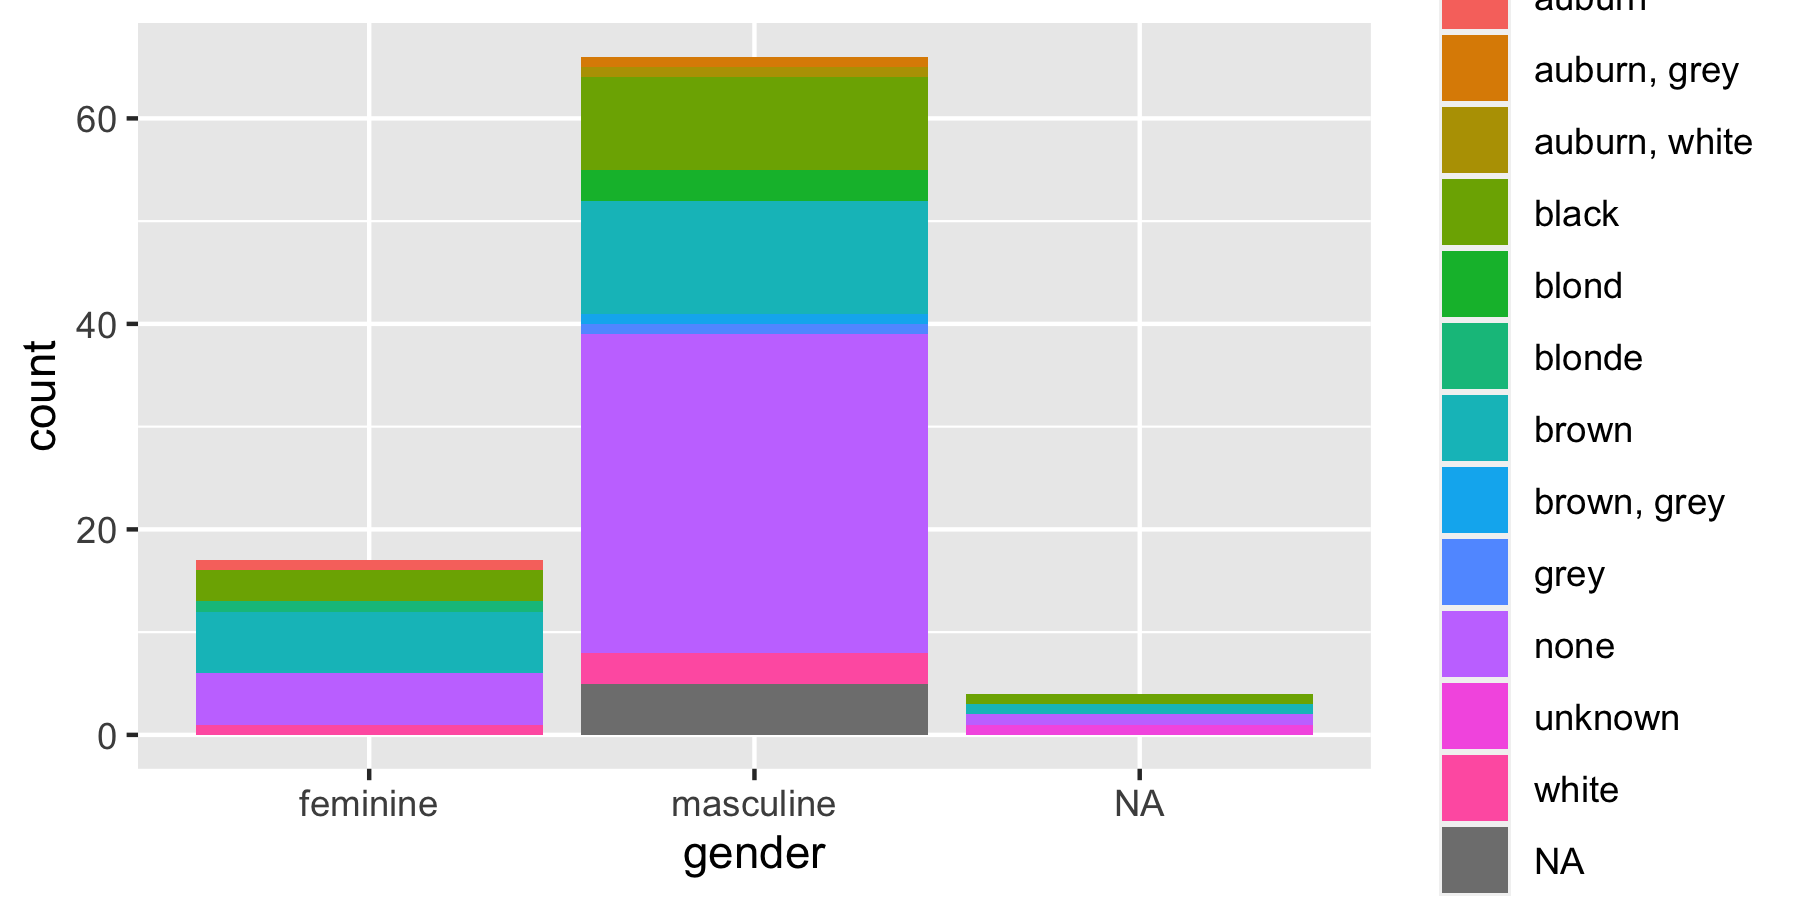
\includegraphics{Lab1_files/figure-latex/unnamed-chunk-5-1.pdf}

\begin{enumerate}
\def\labelenumi{\arabic{enumi}.}
\setcounter{enumi}{3}
\item
  Create a similar visualization, this time showing the distribution of
  review scores (\texttt{review\_scores\_rating}) across neighborhoods.
  In your answer, include a brief interpretation of how Airbnb guests
  rate properties in general and how the neighborhoods compare to each
  other in terms of their ratings.
\item
  Create another informative visualization of your choosing. Be prepared
  to share it with the class -- although the visualization should need
  no explaining!
\end{enumerate}

\hypertarget{instructional-staff-employment-trends}{%
\subsection{Instructional staff employment
trends}\label{instructional-staff-employment-trends}}

The next dataset is about instructional staff employee hiring trends
between 1975 and 2011. The dataset is called \texttt{instructors}. You
can find descriptions of each of the variables in the help file for the
dataset, which you can access by running \texttt{?instructors} in your
Console.

The American Association of University Professors (AAUP) is a nonprofit
membership association of faculty and other academic professionals.
\href{https://www.aaup.org/sites/default/files/files/AAUP_Report_InstrStaff-75-11_apr2013.pdf}{This
report} compiled by the AAUP shows trends in instructional staff
employees between 1975 and 2011, and contains an image very similar to
the one given below.

\begin{enumerate}
\def\labelenumi{\arabic{enumi}.}
\setcounter{enumi}{5}
\item
  Recreate a graph similar to the one above.
\item
  Discuss how you would improve upon this visualization if the main
  objective was to communicate that the proportion of part-time faculty
  have gone up over time compared to other instructional staff
  types.Implement the improvements and provide your improved
  visualization as part of your answer. Also write a few sentences about
  why you chose to make these improvements and how they address the main
  goal stated above.
\end{enumerate}

\end{document}
